%#!platex
\documentclass[a4j,11pt]{jsarticle}
\usepackage{graphicx}

\title{コンパイラ講義ノート}
\author{国島丈生}
\date{2005-06-01}

\newtheorem{theorem}{定理}
\newtheorem{example}{例}
\newtheorem{definition}{定義}

\usepackage{ascmac}	% required for `\screen' (yatex added)
\begin{document}
\maketitle
\section*{練習問題の解答}
\begin{enumerate}
 \item 文脈自由文法
       \[
	string \rightarrow string + string | string - string | 0 | 1 | 2
       | 3 | 4 | 5 | 6 | 7 | 8 | 9
       \]
       について、トークン列$8-2+6$の解析木を示せ。可能なすべての場合を示
       し、自然な式の意味になるものはどれか示せ。

       \begin{center}
	\includegraphics[scale=0.8]{compiler20050525-answer.eps}
       \end{center}

       $+, -$は左結合の演算子であり、括弧がなければ式の左から計算していく
       のが正しい意味になる。したがって、下側の解析木のほうが自然である。
       このように、文法によっては、同じ記号列に対して解析木が2通り以上考
       えられる場合がある。このような文法を{\bfseries 曖昧である}という。
 \item 文脈自由文法$S \rightarrow 0 S 1 | 0 1$はどのような言語を表すか。

       $0$が$n$個($n \geq 1$)並んだ後に$1$が$n$個並んだような文字列すべて
       からなる言語。$0, 1$をそれぞれ$\{, \}$に置き換えてみると、これは対
       応関係のとれた括弧の入れ子を表す。この言語は正則言語ではない例とし
       て有名である。つまり、この言語は正則表現では書けず、またこの言語を
       受理する有限オートマトンも作れない。
\end{enumerate}

\section{文脈自由文法}
文脈自由文法の定義は前回述べた。

\begin{screen}
 \begin{example}
 次の文法は、簡単な算術式を定義するものである。
 \begin{eqnarray*}
  expr & \rightarrow & expr\ op\ expr\ |\ (\ expr\ )\ |\ -\ expr\ |\
   {\bf id} \\
  op & \rightarrow & + | - | * | / 
 \end{eqnarray*}
 \end{example}
\end{screen}

以降の説明では、次のように記法を決めておくことにする。
\begin{enumerate}
 \item 前のほうの英小文字($a, b, c, \cdots$)、演算子記号($+, -, \cdots$)、
       括弧やコンマなどの区切り記号、数字、太字の記号列は終端記号を表す。
 \item 前のほうの英大文字($A, B, C, \cdots$)、$S$ (開始記号)、英小文字の
       イタリック体の名前({\itshape expr}, {\itshape stmt}など)は非終端記
       号を表す。
 \item 後ろのほうの英大文字($X, Y, Z, \cdots$)は非終端記号または終端記号
       を表す。
 \item 後ろのほうの英小文字($x, y, z, \cdots$)は終端記号列を表す。
 \item 小文字のギリシャ文字($\alpha, \beta, \gamma, \cdots$)は、記号列(終
       端記号と非終端記号が混ざっていてよい)を表す。
 \item 最初に現れる生成規則の左辺を開始記号とする。
\end{enumerate}

\subsection{導出}

文法の言語の定義方法にはいくつかあるが、その1つに「生成規則を書き換え規則
と考える」というものがある。つまり、開始記号$S$を$S-$生成規則の右辺の記号
列$\alpha$で置き換え、さらに$\alpha$に含まれる非終端記号を、その記号の生
成規則の右辺で置き換える。この操作を、記号列が終端記号のみになるまで繰り
返す。このようにして得られる終端記号列すべての集合を、その文法の
{\bfseries 言語}という。

\begin{example}\label{ex:derive}
 文法$E \rightarrow E + E | E * E | (E) | -E | {\bf id}$において、$E$を
 右辺の記号列、例えば$-E$で置き換えることができる。このとき、$E$から$-E$
 を{\bfseries 導出する}といい、$E \Rightarrow -E$と表す。□
\end{example}

もう少し形式的に書くと次のようになる。生成規則$A \rightarrow \gamma$を記
号列$\alpha A\beta$に適用して書き換えを行うと$\alpha\gamma\beta$となる。
このとき$\alpha A\beta \Rightarrow \alpha\gamma\beta$と表す。$\alpha_1
\Rightarrow \alpha_2 \Rightarrow \cdots \Rightarrow \alpha_n$のとき、
$\alpha_1 \stackrel{*}{\Rightarrow} \alpha_n$と書く。文法$G$の開始記号を
$S$とするとき、$G$の言語$L(G) = \{w | S \stackrel{*}{\Rightarrow} w\}$で
ある。

$S \stackrel{*}{\Rightarrow} \alpha$のとき、$\alpha$を{\bfseries 文形式}
という。とくに$\alpha$が終端記号のみからなるとき、{\bfseries 文}という。

\subsection{最左導出、最右導出}

例\ref{ex:derive}の文法において、記号列$-({\bf id}+{\bf id})$を導出する方
法はいくつかある。
\[
 E \Rightarrow -E \Rightarrow -(E) \Rightarrow -(E+E) \Rightarrow
  -({\bf id}+E) \Rightarrow -({\bf id}+{\bf id})
\]
\[
 E \Rightarrow -E \Rightarrow -(E) \Rightarrow -(E+E) \Rightarrow
  -(E+{\bf id}) \Rightarrow -({\bf id}+{\bf id})
\]
つまり、文形式の中でどの非終端記号を置き換えるかによって、導出の様子が変
わってくる。これらの導出の中で、必ず文形式の一番左の非終端記号を置き換え
るような導出を{\bfseries 最左導出}、一番右の非終端記号を置き換えるような
導出を{\bfseries 最右導出}という。

\subsection{解析木と導出}

解析木は、導出の様子を(順番を無視して)図示したものと考えられる。したがっ
て、どの解析木も必ず1つの最左導出(または最右導出)と対応づけられる。

\subsection{曖昧な文法}

1つの文に対して2つ以上の解析木が作れる文法を{\bfseries 曖昧である}という。
つまり、曖昧な文法では1つの文に対して最左導出(または最右導出)が2つ以上存
在する。構文解析では2つ以上の解析木ができてしまうのは困るので、曖昧でない
文法に変換したり、ある種の規則を設けて複数の解析木から1つを選ぶようにした
りする。

曖昧さを解消する方法は、あまり体系的にはなっていない。例えば、前回の練習
問題(1)の文法は曖昧であるが、前回の講義中に示した次の文法に変形すれば曖昧
さは解消できる。
\begin{eqnarray*}
 list & \rightarrow & list + digit \\
 list & \rightarrow & list - digit \\
 list & \rightarrow & digit \\
 digit & \rightarrow & 0 | 1 | 2 | 3 | 4 | 5 | 6 | 7 | 8 | 9
\end{eqnarray*}

もう1つ例を挙げよう。
\begin{eqnarray*}
 stmt & \rightarrow & {\bf if}\ (expr)\ stmt\  \\
      & | & {\bf if}\ (expr)\ stmt\ {\bf else}\ stmt \\
      & | & \cdots
\end{eqnarray*}
上に示したのはif文を表す文法である。しかし、図
\ref{fig:ambiguous_grammar}で分かるように、この文法は次の文に対して2つの
解析木を生成するので、曖昧である。
\[
 {\bf if}\ (E_1)\ S_1\ {\bf else}\ {\bf if}\ (E_2)\ S_2\ {\bf else}\ S_3
\]

\begin{figure}[]
 \begin{center}
  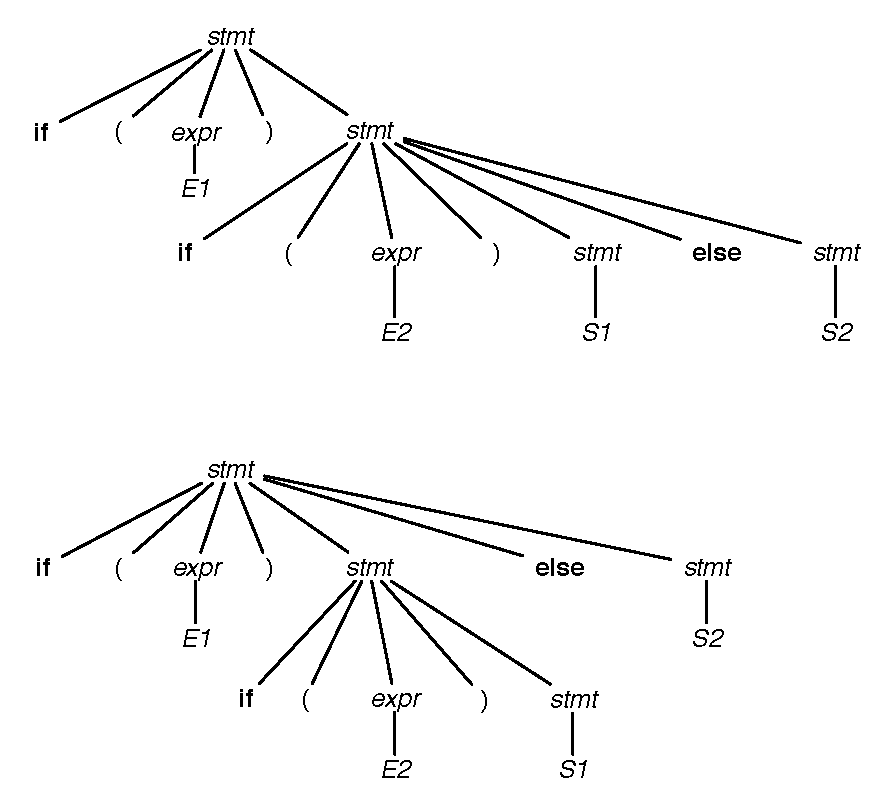
\includegraphics[scale=0.8]{fig4.6.eps}
 \end{center}
 \caption{曖昧な文法に対する2つの解析木}
 \label{fig:ambiguous_grammar}
\end{figure}

このような条件文の文法では普通、「各elseは前のほうにある未対応のthen文の
うち、もっとも近いものと対応する」という規則を設け、曖昧性を解消する。つ
まり図\ref{fig:ambiguous_grammar}の解析木のうち、上のほうを採用する。次の
ように文法を書き換えることで、曖昧さが解消できる。

\begin{eqnarray*}
 stmt & \rightarrow & matched\_stmt \\
      & |           & unmatched\_stmt \\
 matched\_stmt & \rightarrow & {\bf if}\ (expr)\ matched\_stmt\ {\bf
  else}\ matched\_stmt \\
      & |           & \cdots \\
 unmatched\_stmt & \rightarrow & {\bf if}\ (expr)\ stmt \\
                 & |           & {\bf if}\ (expr)\ matched\_stmt\ {\bf
		  else}\ unmatched\_stmt
\end{eqnarray*}

\subsection{左再帰}

$A \stackrel{*}{\Rightarrow} A\alpha$という導出が存在するとき、この文法は
{\bfseries 左再帰}であるという。予測型構文解析法では非終端記号それぞれに
(再帰)関数を定義し、生成規則の通りに関数を呼び出すことで構文解析を進めて
いく。したがって、左再帰の文法では停止しない再帰呼び出しが起こってしまう。
つまり、左再帰の文法は、予測型構文解析では扱えない\footnote{実は、一般に
下向き構文解析法はすべて、左再帰の文法を扱うことができない。}。

もっとも簡単な左再帰の文法は、$A \rightarrow A\alpha$という形の生成規則を
持つものである。ここでは、この形の生成規則を含む左再帰文法を、左再帰では
ない文法に変換する方法のみ示す。左再帰の文法のA-生成規則は、一般に
\[
 A \rightarrow A\alpha_1 | A\alpha_2 | \cdots | A\alpha_m | \beta_1 |
 \beta_2 | \cdots | \beta_n
\]
と書ける。ここで$\beta_i$は$A$以外の記号で始まる記号列である。このとき、
このA-生成規則を次のように変形する。
\begin{eqnarray*}
 A & \rightarrow & \beta_1 A' | \beta_2 A' | \cdots | \beta_n A' \\
 A' & \rightarrow & \alpha_1 A' | \alpha_2 A' | \cdots | \alpha_m A' | \epsilon
\end{eqnarray*}
この文法は、変形前のものと同じ言語を生成し、かつ左再帰を含まない。

\subsection{左端の括り出し}

先に挙げた文法の一部について、再び考える。

\begin{eqnarray*}
  unmatched\_stmt & \rightarrow & {\bf if}\ (expr)\ stmt \\
                 & |           & {\bf if}\ (expr)\ matched\_stmt\ {\bf
		  else}\ unmatched\_stmt
\end{eqnarray*}

トークン{\bfseries if}を読み込んだとき、どちらの生成規則を用いて
{\itshape unmatched\_stmt}を書き換えればよいかはまだ判断できない。ずっとトー
クン列を読んでいって、{\bfseries else}が出てきて初めて、下の生成規則を適
用すればよいということが分かる。このとき、処理の逆戻り(バックトラック)が
発生する可能性が高く、効率が悪くなる。

このような場合には、次のように左端を括り出すと、処理の逆戻りが発生しなく
なる。
\begin{eqnarray*}
 unmatched\_stmt & \rightarrow & {\bf if}\ (expr)\ unmatched\_stmt' \\
 unmatched\_stmt' & \rightarrow & stmt \\
                  & |           & matched\_stmt\ {\bf else}\ unmatched\_stmt
\end{eqnarray*}

\subsection{予測型構文解析}

文法$G$について予測型構文解析を行うには、$G$が次のような制限を満たしてい
なければならない。
\begin{enumerate}
 \item $G$は曖昧でなく、かつ左再帰ではない。
 \item 生成規則$A \rightarrow \alpha_1 | \alpha_2 | \cdots | \alpha_n $に
       ついて、現在の入力記号$a$のみからどの生成規則で$A$を書き換えればよ
       いか、一意に決定できなければならない。
\end{enumerate}
左端の括り出しとは、2番目の制限を満たすように文法を変形することに他ならな
い。ただし、左端の括り出しだけでは不十分な場合があり、もう少し精密に議論
しなければならない。この部分は次週以降に譲る。

\section{文脈自由文法の限界}

言語$L = \{wcw | w \in (a | b)^* \}$は「$c$の前後に同じ文字列$w$が出現す
るような言語」であり、プログラミング言語での「変数を使うときには、それよ
り前に宣言をしておかなければならない」という決まりを抽象化したものと言え
る。ところが、実は$L$は文脈自由文法では表現できない。つまり、変数を使う前
に宣言されているか検査するのは、構文解析フェーズでは行うことができない。
実際、この検査は、意味解析フェーズで行われている。

このように、プログラミング言語の制限には構文解析フェーズで検査できないも
のがあり、それらは意味解析フェーズで検査されることが多い。

\section*{練習問題}

\begin{enumerate}
 \item 次の文法を考える。
       \begin{eqnarray*}
	S & \rightarrow & A1B \\
	A & \rightarrow & 0A | \epsilon \\
	B & \rightarrow & 0B | 1B | \epsilon
       \end{eqnarray*}
       この文法に対し、文字列$00101$の最左導出、最右導出を示せ。
 \item 算術式に対する文法
       \begin{eqnarray*}
	E & \rightarrow & E + T | T \\
	T & \rightarrow & T * F | F \\
	F & \rightarrow & (E) | {\bf id}
       \end{eqnarray*}
       を、左再帰でないように変形せよ。
\end{enumerate}

\end{document}
